\documentclass[../report.tex]{subfiles}
\graphicspath{{\subfix{../image/}}}

\begin{document}

\subsection{Multiplexer-board for IR-sensor interfacing}
As has been discussed in the previous section, multiplexers have to be used in order to be 
able to interface with all the analog outputs of the IR-sensor arrays.
At least 16 pins needs to be routed to one or two ADC pins. For this, the CD4051B 8 channel multiplexer 
by Texas Instruments was chosen (\url{https://www.ti.com/lit/ds/symlink/cd4051b.pdf?ts=1702330047608&ref_url=https%253A%252F%252Fwww.startpage.com%252F}).

\begin{figure}[h!]
    \centering
    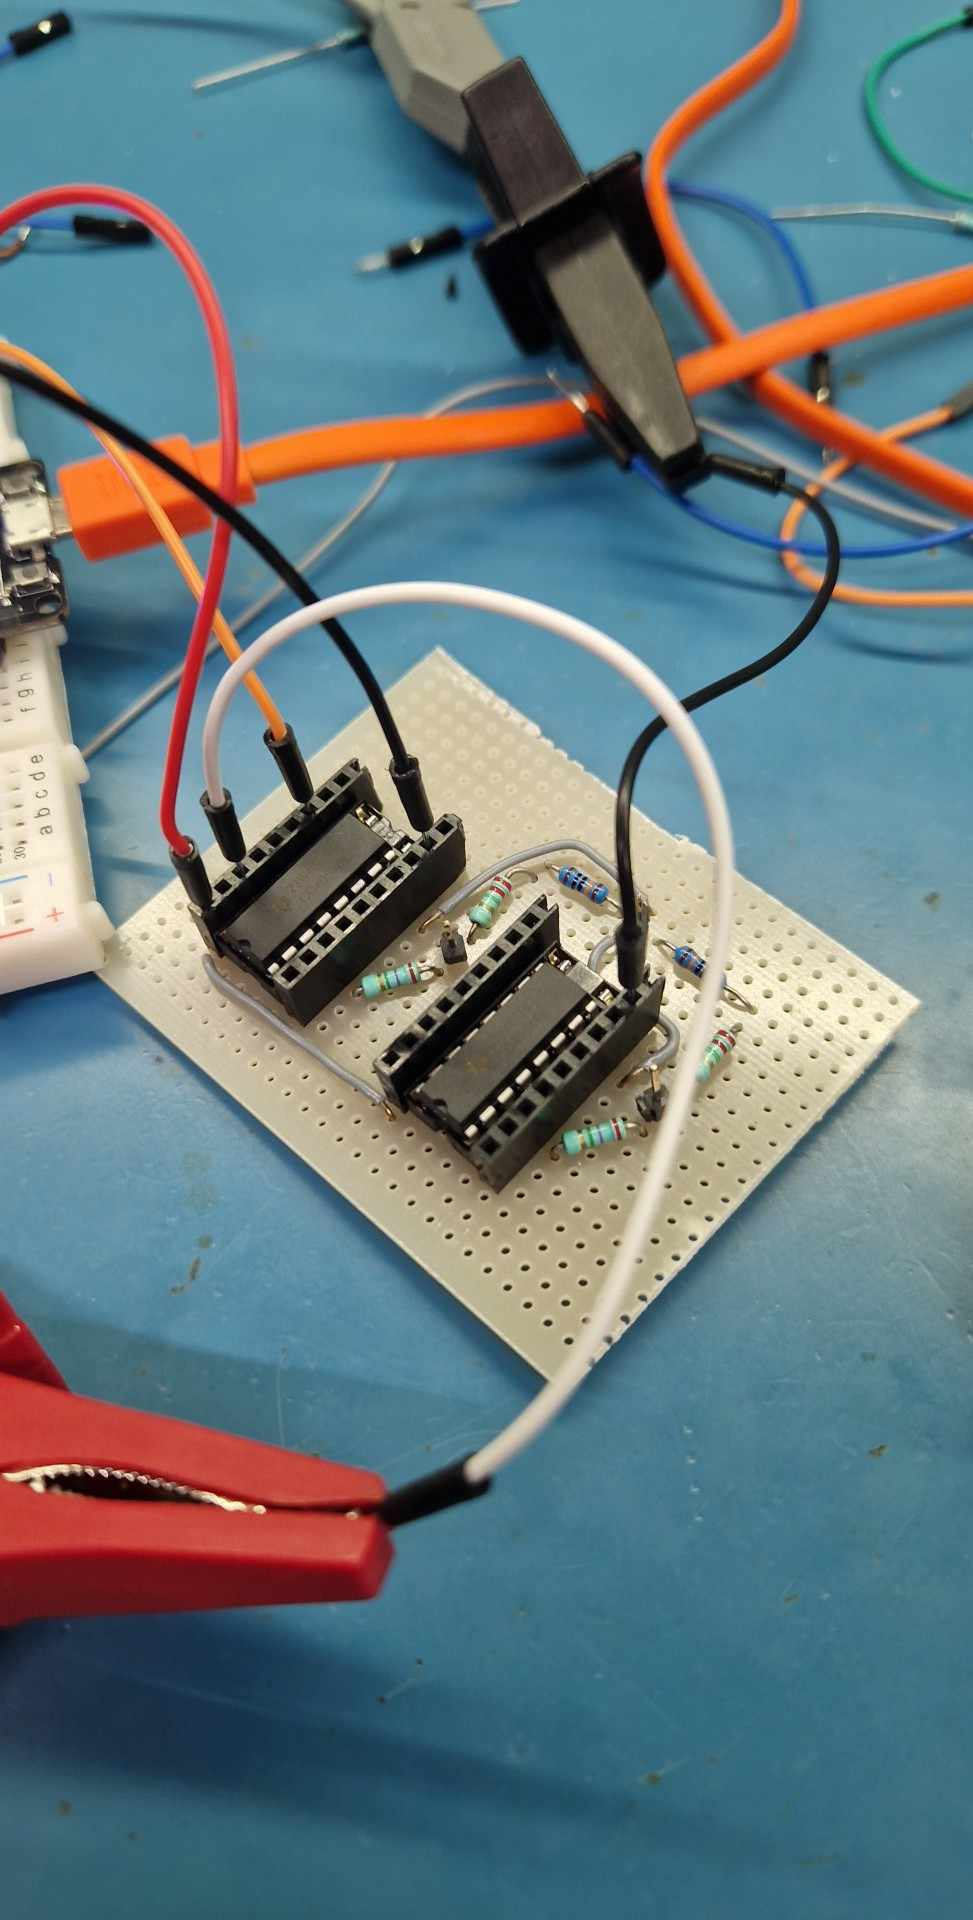
\includegraphics[width=0.2\textwidth]{multiplexerboard.jpg}
    \caption{Multiplexers for analog IR-sensor arrays}
 \end{figure}

Two of them allow to cover all 16 pins. However, as the output of the analog IR-sensors
is in the range of 0 to 5V and the input range of the ADC of the chosen microcontroller's ADC
is just 150mV to 2450mV the output has to divided down. This is done with output voltage of each
multiplexer.

The shown board implements the functionality. The resistors are chosen so that they add up to several
Mega-Ohm - so current is not a problem. As always calculations were made with MATLAB and extensive
testing has been done to follow the engineering method.


\end{document}